\documentclass[11pt,a4paper]{article}
\usepackage[margin=2.5cm]{geometry}
\usepackage{amsmath,amssymb,amsthm}
\usepackage{booktabs}
\usepackage{array}
\usepackage{tabularx}
\usepackage{xcolor}
\usepackage{tcolorbox}
\tcbuselibrary{skins,breakable}
\usepackage{hyperref}
\usepackage[numbers,sort&compress]{natbib}
\bibliographystyle{unsrtnat}
\hypersetup{colorlinks=true,linkcolor=blue!60!black,urlcolor=blue!60!black}
\usepackage{enumitem}
\usepackage{tikz}
\usetikzlibrary{arrows.meta,positioning,shapes.geometric,calc}
\usepackage{microtype}

%─── colour palette (matches polynomial cheatsheet) ──────────────────────────
\definecolor{boxblue}{RGB}{220,235,255}
\definecolor{boxorange}{RGB}{255,240,210}
\definecolor{boxgreen}{RGB}{220,245,220}
\definecolor{boxgray}{RGB}{240,240,240}

%─── convenience commands ────────────────────────────────────────────────────
\newcommand{\term}[1]{\textbf{#1}}
\newcommand{\PSC}{\textsc{psc}}
\newcommand{\MDL}{\textsc{mdl}}
\newcommand{\PI}{\textsc{pi}}
\newcommand{\SM}{$\mathrm{SU}(3){\times}\mathrm{SU}(2){\times}\mathrm{U}(1)$}
\newcommand{\lean}[1]{\texttt{#1}}
\newcommand{\CatAL}{\ensuremath{\mathbf{A}_{\rm Lean}}}

\newtheorem*{remark}{Remark}

\title{\textbf{Perfect Self-Containment and MDL}\\[6pt]
\large Why the Universe Has to Select Itself\\[4pt]\normalsize\textit{UGP Physics Tutorial Series}
\\[2pt]\small\href{https://doi.org/\TutorialDOI}{doi.org/\TutorialDOI}}
\author{Nova Spivack\\[4pt]
\normalsize
\href{https://novaspivack.com/research}{novaspivack.com/research}\\[2pt]
\small Full monograph (P48):
\href{https://doi.org/10.5281/zenodo.20560550}{doi.org/10.5281/zenodo.20560550}
}
\newcommand{\TutorialDOI}{10.5281/zenodo.20657895}
\date{2026}

\begin{document}
\setcounter{tocdepth}{2}
\maketitle
\tableofcontents
\newpage

\begin{tcolorbox}[colback=blue!6,colframe=blue!40!black,
  title=\textbf{UGP Physics Tutorial Series}]
\textbf{Prerequisites (read first):} \href{https://doi.org/10.5281/zenodo.20657889}{\emph{The GTE Polynomial: A Step-by-Step Cheat Sheet}} $\cdot$ \href{https://doi.org/10.5281/zenodo.20657913}{\emph{From the Arithmetic Substrate to Particle Masses}}\\[4pt]
\textbf{Next tutorials:} \href{https://doi.org/10.5281/zenodo.20657876}{\emph{How MDL Selects the 19-Bit Polynomial}}\\[4pt]
\textbf{See also:} \href{https://doi.org/10.5281/zenodo.20657885}{\emph{The $\Phi_{\rm MDL}$ Field}}
\end{tcolorbox}

\begin{tcolorbox}[colback=boxgreen,colframe=green!50!black,
  title=\textbf{Claim-Strength Taxonomy}]
Throughout this tutorial, results are labeled with a confidence grade:
\begin{itemize}[itemsep=2pt]
  \item \textbf{$\mathbf{A}_{\rm Lean}$ (CatAL)} --- Machine-certified in Lean~4 with zero \texttt{sorry} and zero custom axioms.  Independently verifiable by anyone with Lean installed.
  \item \textbf{A/D (CatAD)} --- Analytically derived with full derivation, computationally confirmed.  Not yet machine-certified.
  \item \textbf{A (CatA)} --- Analytically derived; derivation complete but not independently machine-certified.
  \item \textbf{A/D (conditional)} --- Derived under a named, stated premise; the premise is itself an open problem or a CatB assumption.
  \item \textbf{B (CatB)} --- A stated working hypothesis or structural premise; not yet derived.
\end{itemize}
\end{tcolorbox}


%═════════════════════════════════════════════════════════════════════════════
\section{The Puzzle}
\label{sec:puzzle}
%═════════════════════════════════════════════════════════════════════════════

\begin{tcolorbox}[colback=boxblue,colframe=blue!40!black,
  title=The central question]
Why do the laws of physics have the specific values they do?
Who — or what — chose them?
\end{tcolorbox}

\subsection{The mystery of the 25 dials}

The Standard Model of particle physics is the most precise physical theory ever
constructed.  It predicts the magnetic moment of the electron to 12 decimal places,
describes the strong force, the weak force, and electromagnetism, and accounts for
essentially every subatomic observation ever made.

But it has a dirty secret: it comes with \textbf{25 free parameters} — 25 numerical dials
that nobody knows how to set from first principles.  The mass of the electron is just
what it is.  The number of particle generations (three) is just what it is.
The fine-structure constant $\alpha \approx 1/137$ is just what it is.
You measure them, you write them into the theory, and the theory works.
But the theory cannot explain \emph{why} those values rather than others.

This is a deep problem.  Imagine an architect who designs a beautiful building but whose
blueprint requires 25 arbitrary numbers — the ratio of ceiling height to door width,
the exact colour of each brick — that have no internal reason.  The building stands, but
it was designed around coincidences, not principles.  Our universe is like that building.

\subsection{The three standard answers — and why none is fully satisfying}

\paragraph{Answer 1: They are brute facts.}
The coupling constants just happen to be what they are.
There is no deeper explanation.
This is honest, but it amounts to saying the question has no answer — not a theory at all.

\paragraph{Answer 2: Anthropic reasoning.}
Perhaps there are infinitely many universes with different values of the constants.
We live in one where the constants happen to permit stars, atoms, and observers.
This might be true, but it provides no prediction and no principle — it explains any set
of constants equally well (or equally poorly).

\paragraph{Answer 3: String landscape.}
String theory predicts something like $10^{500}$ possible universes, each with different
laws.  But the theory offers no mechanism to select our universe from that landscape.
It replaces 25 unexplained numbers with an unexplained selection event.

\medskip

\begin{tcolorbox}[colback=boxorange,colframe=orange!60!black,
  title=The key observation]
Every proposed answer either defers to something external (another theory that must
itself be explained) or accepts the parameters as unexplained primitives.
Neither constitutes a final answer.

The question is: can the universe \emph{explain its own laws} from the inside?
\end{tcolorbox}

\subsection{The PSC approach: no outside}

Perfect Self-Containment (\PSC) is the formal statement that the universe has no
``outside'' from which its laws could be selected.  The laws, their description, and
everything needed to run the physics must all be \emph{internal} — self-contained.

This sounds almost tautological: of course the universe contains everything.  But the
formal consequences are surprisingly powerful.  If you take the requirement seriously
and work out what it implies step by step, you get a filter that eliminates almost
every possible physics, leaving only one candidate: the actual Standard Model.

This tutorial explains how that works.

%═════════════════════════════════════════════════════════════════════════════
\section{Perfect Self-Containment: The Idea}
\label{sec:psc}
%═════════════════════════════════════════════════════════════════════════════

\begin{tcolorbox}[colback=boxblue,colframe=blue!40!black,
  title=One-sentence version of PSC]
A self-contained universe must be able to compute all its own predictions,
remain stable without external fine-tuning, support persistent structures,
allow those structures to communicate, and maintain internal consistency
under quantum corrections — all at once, with no external assistance.
\end{tcolorbox}

\subsection{The five requirements}

\PSC\ is formalized as five \term{Layer~I axioms} — five conditions that any universe
with no outside must satisfy.  Think of them as a checklist.  A proposed physics either
passes all five or fails self-containment.

\medskip

\textbf{Analogy.}  Imagine a self-contained city-state that must never import anything.
It must be able to grow its own food, generate its own power, educate its own citizens,
communicate internally, and balance its own economy.  Each requirement is minimal:
remove any one and the city becomes dependent on something external.
The five PSC axioms work the same way for a universe.

\bigskip

\begin{tcolorbox}[colback=boxgreen,colframe=green!50!black,
  title=Axiom 1 — RC: Reflexive Closure,breakable]
\textbf{Formal statement:} The theory computes its own S-matrix (all scattering
amplitudes, all predictions) up to a UV closure scale, with anomaly cancellation,
unitarity, and UV consistency all internally satisfied.  No external regulator required.

\medskip
\textbf{Plain English:} The laws must be able to predict everything within their own
domain without asking for outside help.  A theory that breaks down at some energy scale
— requiring an external ``patch'' to remove infinities — has secretly outsourced part
of its physics.  That extra patch is an external input, violating self-containment.

\medskip
\textbf{Analogy:} A self-contained calculator must give an answer for every valid input.
A calculator that says ``call an external service for inputs over 1{,}000'' is not
self-contained.

\medskip
\textbf{What it kills:} Any gauge theory with uncanceled quantum anomalies — internal
inconsistencies in the gauge symmetry structure that require external UV physics to fix.
\end{tcolorbox}

\bigskip

\begin{tcolorbox}[colback=boxgreen,colframe=green!50!black,
  title=Axiom 2 — NM*: Structural Stability,breakable]
\textbf{Formal statement:} The qualitative character of the universe (unbroken gauge
group, particle spectrum, chiral structure, sign of the baryon asymmetry) is stable
under small changes to the coupling constants — it does not flip to something
qualitatively different for generic parameter values.

\medskip
\textbf{Plain English:} If the type of physics you get changes drastically when you
nudge a parameter by a tiny amount, then something external must be holding that
parameter at the exact right value.  A self-contained universe must work robustly, not
only at one fine-tuned point.

\medskip
\textbf{Analogy:} A properly engineered bridge works for a wide range of loads.
A bridge that collapses if the temperature changes by 0.01$^\circ$C requires a
thermostatic life-support system to keep it standing — it is not self-contained.

\medskip
\textbf{What it kills:} Grand Unified Theories based on SU(5), SO(10), or $E_6$
--- their symmetry-breaking pattern flips to a qualitatively different phase when
parameters cross a boundary, requiring external stabilization.
For example, in SU(5) GUT the breaking chain $\mathrm{SU}(5) \to \mathrm{SU}(3) \times
\mathrm{SU}(2) \times \mathrm{U}(1)$ requires the Higgs self-coupling to fall within a
window of relative width $\lesssim 10^{-3}$; outside that window the symmetry either
fails to break or breaks to the wrong subgroup, requiring an external mechanism to hold
the parameter on target.
Also kills theories with too few generations ($N_{\rm gen} < 3$), where
CP-violation is insufficient to produce a matter--antimatter asymmetry for generic
initial conditions.
\end{tcolorbox}

\bigskip

\begin{tcolorbox}[colback=boxgreen,colframe=green!50!black,
  title=Axiom 3 — TV: Thermodynamic Viability,breakable]
\textbf{Formal statement:} Stable composite structures (atoms, nuclei, molecules) exist
and persist over cosmological timescales.

\medskip
\textbf{Plain English:} The universe must support persistent physical structures.
Without them, the universe has no memory, no substrate to carry information, and no way
to instantiate its own laws beyond an instant.  A universe in permanent thermal
equilibrium everywhere cannot record anything about itself.

\medskip
\textbf{Analogy:} A library that stores no books contains no knowledge.  For the
universe to carry information about its own laws, it needs structures that last.

\medskip
\textbf{What it kills:} Any universe with only massless unconfined particles and no
attractive force strong enough to form bound states.  If nothing binds, nothing persists.
\end{tcolorbox}

\bigskip

\begin{tcolorbox}[colback=boxgreen,colframe=green!50!black,
  title=Axiom 4 — SA: Semantic Admissibility,breakable]
\textbf{Formal statement:} Information-bearing subsystems exist \emph{and} long-range
interactions enable signal propagation, information storage, and energy dissipation.
At minimum, a massless mediator sector (a U(1) gauge boson — i.e., a photon) is required.

\medskip
\textbf{Plain English:} TV requires persistent structures; SA requires that those
structures can \emph{communicate}.  Without a massless particle (like the photon),
all forces fall off exponentially over distance.  No signal can propagate across the
universe; no part of the universe can ``know'' about another part.  Such a universe
cannot carry semantic content about its own state.

\medskip
\textbf{Analogy:} A network of isolated computers, each with a hard drive but no
network connection, cannot collectively carry information that transcends any
individual node.  The photon is the universe's network cable.

\medskip
\textbf{What it kills:} Any purely massive gauge theory (no massless photon).
All forces are short-range; information processing shuts down below the lightest
particle mass.
\end{tcolorbox}

\bigskip

\begin{tcolorbox}[colback=boxgreen,colframe=green!50!black,
  title=Axiom 5 — AC: Anomaly Consistency,breakable]
\textbf{Formal statement:} All gauge anomalies cancel: the gauge symmetry remains
quantum-mechanically consistent.  No chiral anomalies appear in gauge currents.

\medskip
\textbf{Plain English:} The gauge symmetries that protect the universe from unphysical
degrees of freedom must survive when quantum corrections are applied.  An
``anomalous'' gauge theory is self-defeating: quantum effects secretly destroy the very
symmetry that makes the theory sensible.  That destruction requires external UV physics
to repair it.

\medskip
\textbf{Analogy:} A self-consistent accounting system must balance at every level.
If quantum corrections accumulate like hidden debt that requires external bailouts, the
system is not self-contained.

\medskip
\textbf{What it kills:} Gauge theories with wrong hypercharge assignments — where the
chiral anomaly does not cancel between left- and right-handed fermions.  Strikingly,
the actual hypercharge assignments of quarks and leptons in the Standard Model are
the \emph{unique} choice that makes the anomaly cancel.
\end{tcolorbox}

\bigskip

\begin{center}
\begin{tabular}{@{}lll@{}}
\toprule
\textbf{Axiom} & \textbf{Plain name} & \textbf{What it prevents} \\
\midrule
RC & Reflexive Closure  & Needing external UV regulators \\
NM* & Structural Stability & Requiring fine-tuned parameter stabilization \\
TV & Thermodynamic Viability & A structureless, memory-free universe \\
SA & Semantic Admissibility & A universe that cannot communicate internally \\
AC & Anomaly Consistency & Gauge symmetries broken by quantum corrections \\
\bottomrule
\end{tabular}
\end{center}

%═════════════════════════════════════════════════════════════════════════════
\section{What PSC Forces: The Two-Layer Structure}
\label{sec:twolayer}
%═════════════════════════════════════════════════════════════════════════════

\begin{tcolorbox}[colback=boxblue,colframe=blue!40!black,
  title=The punchline]
Start with all $34{,}560$ possible universes (compact gauge theories in four
dimensions).  Apply the five \PSC\ axioms in sequence.  Only 12 survive.
All 12 have exactly the Standard Model gauge structure.
\end{tcolorbox}

\subsection{The candidate universe space}

To make the filter concrete, you need to specify what you are filtering.
The relevant space is \term{TSpace}: the collection of all
four-dimensional renormalizable gauge quantum field theories with compact gauge groups
and chiral matter (the class to which the Standard Model belongs).

Within TSpace, there are $34{,}560$ candidate universes — all compact gauge groups of
rank up to 4, with anomaly-consistent chiral matter representations.
This is a large but finite and fully enumerable set.  The five axioms are then applied
as a sieve.

\subsection{The funnel: 34,560 \texorpdfstring{$\to$}{to} 12}

\begin{center}
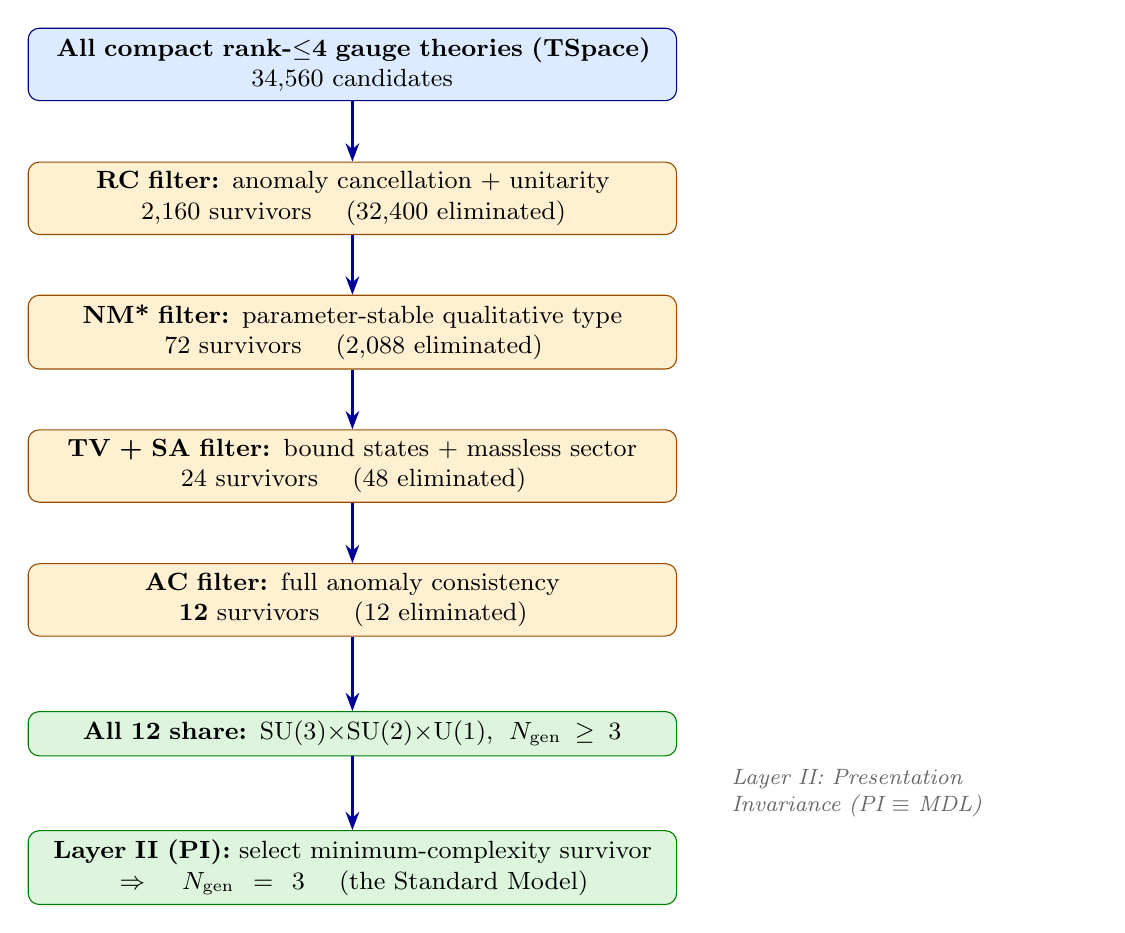
\begin{tikzpicture}[
  box/.style={
    draw, rounded corners=4pt,
    text width=8cm, align=center,
    minimum height=1.6em, font=\small,
    fill=boxblue, draw=blue!50!black
  },
  redbox/.style={
    draw, rounded corners=4pt,
    text width=8cm, align=center,
    minimum height=1.6em, font=\small,
    fill=boxorange, draw=orange!60!black
  },
  greenbox/.style={
    draw, rounded corners=4pt,
    text width=8cm, align=center,
    minimum height=1.6em, font=\small,
    fill=boxgreen, draw=green!50!black
  },
  arrow/.style={-Stealth,thick,blue!60!black},
  note/.style={font=\footnotesize\itshape,text=gray!80!black,text width=4.5cm,align=left}
]
\node[box] (start) at (0,0)
  {\textbf{All compact rank-$\leq$4 gauge theories (TSpace)}\\
   $34{,}560$ candidates};

\node[redbox] (rc) at (0,-1.7)
  {\textbf{RC filter:} anomaly cancellation + unitarity\\
   $2{,}160$ survivors \quad ($32{,}400$ eliminated)};

\node[redbox] (nm) at (0,-3.4)
  {\textbf{NM* filter:} parameter-stable qualitative type\\
   $72$ survivors \quad ($2{,}088$ eliminated)};

\node[redbox] (tvsa) at (0,-5.1)
  {\textbf{TV + SA filter:} bound states + massless sector\\
   $24$ survivors \quad ($48$ eliminated)};

\node[redbox] (ac) at (0,-6.8)
  {\textbf{AC filter:} full anomaly consistency\\
   $\mathbf{12}$ survivors \quad ($12$ eliminated)};

\node[greenbox] (result) at (0,-8.5)
  {\textbf{All 12 share:}
   $\mathrm{SU}(3){\times}\mathrm{SU}(2){\times}\mathrm{U}(1)$,
   \;$N_{\rm gen} \geq 3$};

\node[greenbox] (l2) at (0,-10.2)
  {\textbf{Layer II (PI):} select minimum-complexity survivor\\
   $\Rightarrow\;N_{\rm gen} = 3$ \quad (the Standard Model)};

\draw[arrow] (start) -- (rc);
\draw[arrow] (rc) -- (nm);
\draw[arrow] (nm) -- (tvsa);
\draw[arrow] (tvsa) -- (ac);
\draw[arrow] (ac) -- (result);
\draw[arrow] (result) -- (l2)
  node[note,right=47mm,midway] {Layer II: Presentation\\Invariance (PI $\equiv$ MDL)};
\end{tikzpicture}
\end{center}

\subsection{Layer I vs.\ Layer II}

The two layers do different things:

\begin{center}
\begin{tabular}{@{}p{2.5cm}p{4.5cm}p{5cm}@{}}
\toprule
\textbf{Layer} & \textbf{What it does} & \textbf{How} \\
\midrule
\textbf{Layer I}
  & \emph{Eliminates} theories that are internally inconsistent
  & Applies the five hard \PSC\ axioms (RC, NM*, TV, SA, AC) as consistency tests \\[8pt]
\textbf{Layer II}
  & \emph{Selects} among the survivors
  & Picks the minimum-complexity theory using Presentation Invariance (PI $\equiv$ MDL) \\
\bottomrule
\end{tabular}
\end{center}

\medskip
Layer I does not pick a winner — it is a filter that kills losers.  Layer II is
the selection principle that identifies a unique winner among the survivors.

\subsection{The result: machine-certified}

The 12-survivor count is machine-certified in Lean 4:
\lean{psc\_layer\_i\_catal\_bundle} (ugp-lean, zero sorry, zero custom axioms)
bundles the per-filter cardinality theorems confirming each elimination step.

\begin{tcolorbox}[colback=boxorange,colframe=orange!60!black,
  title=Two-Layer PSC Theorem (from P48~\cite{SpivackGTECompleteFramework} §3.3)]
\begin{enumerate}[leftmargin=1.5em,itemsep=4pt]
\item \textbf{Layer I:} The five \PSC\ axioms (RC, NM*, TV, SA, AC) restrict the
  survivor set within TSpace to exactly 12 theories, all of gauge structure
  $\mathrm{SU}(3){\times}\mathrm{SU}(2){\times}\mathrm{U}(1)$ with
  $N_{\rm gen} \geq 3$.\\
  \textit{Conditional on: TSpace domain restriction + PSC axiom package.}

\item \textbf{Layer II:} Among the 12 Layer~I survivors, Presentation Invariance (PI)
  selects the unique minimizer of Kolmogorov complexity:
  the theory with $N_{\rm gen} = 3$.\\
  \textit{Conditional on: Generation-Extension Monotonicity Assumption.}
\end{enumerate}
\end{tcolorbox}

\subsection{Why not more or fewer generations?}

It is worth pausing on the $N_{\rm gen} = 3$ result, because it is one of the
deepest puzzles in particle physics.  Why three generations of quarks and leptons?
Why not one or five?

Layer II gives an answer via four \emph{independent} mechanisms that all agree:

\begin{enumerate}[leftmargin=2em,itemsep=6pt]
\item \textbf{Orbit depth (Lean-certified):}
The dynamical structure of the GTE orbit has depth exactly 3.
The first generation is a ``Garden of Eden'' state — it has no predecessor under
the orbit dynamics.  The orbit depth forces the generation count.

\item \textbf{QCD beta function:}
The sign and integrality of the QCD running coupling requires $N_{\rm gen} \in \{3, 6, \ldots\}$.
Layer II then selects the minimum.

\item \textbf{PSC Layer II optimality:}
Among the 12 survivors, adding a generation always strictly increases the
description length of the theory.  So $N_{\rm gen} = 3$ is the PSC-minimal choice.

\item \textbf{Cosmological constant bracket:}
$N_{\rm gen} = 3$ is the unique positive integer for which two independent routes
to the cosmological constant both bracket the observed value.
At $N_{\rm gen} = 2$ or $4$ the bracket fails.
\end{enumerate}

\begin{tcolorbox}[colback=boxblue,colframe=blue!40!black,
  title={Remark: convergence, not coincidence}]
Multiple independent mechanisms with different mathematics all point to the same integer.
This is the structural signature of a genuine derivation.
Seven independent structural constraints (PSC enumeration, DPP dimensional split,
CMCA orbit count, TPC hierarchy depth, Gorard dimension relation, GTE cascade, and
\MDL-minimal orbit structure) are simultaneously machine-certified in a single bundle
\mbox{(\lean{ngen\_universality\_seven\_constraints}, \CatAL)}, with an eighth
constraint conditional on the carrier-pricing identification
\mbox{(\lean{ngen\_universality\_master}, \CatAL)}.
\end{tcolorbox}

%═════════════════════════════════════════════════════════════════════════════
\section{Presentation Invariance and MDL}
\label{sec:pi_mdl}
%═════════════════════════════════════════════════════════════════════════════

\begin{tcolorbox}[colback=boxblue,colframe=blue!40!black,
  title=The key identification]
Presentation Invariance (\PI) — the Layer~II \PSC\ axiom — is exactly equivalent
to Minimum Description Length (\MDL).  Not analogous to it; \emph{identical} to it.
\end{tcolorbox}

\subsection{What Presentation Invariance says}

Here is the core idea: a self-contained universe cannot have its physics depend on
\emph{how it is described}.

Think about what that means.  If you change the coordinates you use to write down a
theory — relabeling fields, choosing a different basis for the gauge group, changing
your parameterization — the physical predictions cannot change.  That is just a
repharsing, like translating a sentence from English to French.  The sentence says
the same thing; only the representation differs.

Presentation Invariance (\PI) formalizes this.  It has two components:

\begin{enumerate}[leftmargin=2em,itemsep=4pt]
\item \textbf{Invariance:} Any two presentations of the same physical theory (related
  by field redefinitions, basis changes, or reparameterizations that preserve all
  observable predictions) have the same complexity.

\item \textbf{Selection:} Among all PSC-consistent theories, the PSC-optimal theory
  is the one with minimum complexity.
\end{enumerate}

\subsection{Why PI is forced by self-containment}

Without PI, you have a problem.  If the complexity measure depended on how you presented
the theory, then ``which presentation to use'' would be an external choice that carries
information not generated by the theory itself.  That free choice — the description
language you pick — would be an external input.  External inputs violate PSC.

So if PSC holds, the complexity measure must be presentation-invariant.  And the unique
presentation-invariant measure of the complexity of an object is \term{Kolmogorov
complexity}: the length of the shortest program that generates a complete description of
the object.  Kolmogorov complexity depends on the information content, not on how you
chose to express it.

\subsection{Why PI is exactly MDL}

Minimum Description Length (\MDL) says: given a set of phenomena to explain, pick the
theory with the shortest description of those phenomena.

In physics:
\begin{itemize}[itemsep=2pt]
  \item The ``phenomena'' are all observable predictions (S-matrix elements).
  \item The ``description'' is the Lagrangian of the theory.
  \item ``Shortest description'' = minimum Kolmogorov complexity $K$.
\end{itemize}

So PI (select the minimum-$K$ theory from the PSC-consistent set) and MDL
(select the minimum-$K$ hypothesis consistent with the data) are the \emph{same
instruction}, stated in different vocabularies.  The data is the S-matrix; consistency
means passing all five Layer~I axioms.

\begin{tcolorbox}[colback=boxorange,colframe=orange!60!black,
  title=PI \texorpdfstring{$\equiv$}{=} MDL: worked analogy,breakable]
\textbf{Situation:} Two programmers, Alice and Bob, each write a function that
computes the same output table.  Alice's program is 50 lines; Bob's is 5 lines.
Both are correct.

\textbf{The question:} Which one does the universe ``use''?

\textbf{The PSC answer:} If the universe is self-contained, the choice of program
cannot matter — both compute identical physics.  A self-contained system cannot care
about the presentation.  But then: which program are we \emph{actually} running?

\textbf{The resolution:} If the universe cannot distinguish presentations, but must
pick one, then by PI it must pick the one with minimum description length — the one
that requires the fewest bits to specify.  That is Bob's 5-line program.  Not because
brevity is beautiful, but because any longer description contains redundant bits that
could only have been placed there by an external choice.  External choices violate PSC.
MDL is the only selection rule consistent with having no outside.
\end{tcolorbox}

\subsection{Why the regress terminates here}

A skeptic might ask: ``But why MDL?  Why not a different selection principle?''
In general, this is a fair question — MDL is not self-justifying on its own.
But within PSC, the regress chain terminates cleanly:

\bigskip
\begin{center}
\renewcommand{\arraystretch}{1.6}
\begin{tabular}{@{}p{2.5cm}p{0.3cm}p{9cm}@{}}
``Why MDL?'' & $\Rightarrow$ & Because PSC forces PI, and PI is MDL in physics vocabulary. \\
``Why PI?'' & $\Rightarrow$ & Because self-containment requires presentation independence.
  A complexity measure that depends on the presentation would let the description
  language in as an external input — violating self-containment. \\
``Why PSC?'' & $\Rightarrow$ & Because a fundamental theory has no outside.
  This is the definition of ``fundamental.'' \\
\end{tabular}
\end{center}

\bigskip

The chain terminates at PSC because PSC is the formal content of the statement
``this theory is fundamental.''  The regress stops here for the same reason that
the regress of physical causation stops at the laws of physics.

\subsection{Lean evidence}

The PI $\equiv$ MDL identification is established analytically in the NEMS foundational
programme (CatAD status).  The closest machine-certified result
demonstrating it in action is:

\begin{tcolorbox}[colback=boxgreen,colframe=green!50!black,
  title={Lean result: MDL-minimizing physical coupling}]
\lean{op9\_catal\_unconditional} (ugp-lean, zero sorry, zero custom axioms):

The SRRG fixed point $g^* = 1/\varphi$, where $\varphi = (\sqrt{5}-1)/2$ is the
golden ratio, is the unique coupling that simultaneously minimizes the MDL cost
function and satisfies the GTE polynomial self-consistency equation
$g = p(g, g, g)$ over $\mathbb{R}$.

This result requires no external input, no free parameters, and no reference to
measured SM parameters.  The Higgs VEV $v = 246.16$~GeV is derived from $g^*$.
\end{tcolorbox}

This theorem is PI $\equiv$ MDL in action: the physical coupling is not a free
parameter inserted from outside.  It is the unique minimizer of the MDL cost,
which is the unique presentation-invariant measure, which is what PI requires.

%═════════════════════════════════════════════════════════════════════════════
\section{MDL's Three Roles in the Theory}
\label{sec:mdl_roles}
%═════════════════════════════════════════════════════════════════════════════

\begin{tcolorbox}[colback=boxblue,colframe=blue!40!black,
  title=Overview]
MDL appears at three levels in GTE.  These are \emph{not} three separate invocations
of the same external principle.  They are three manifestations of one global
self-consistency requirement at three scales of physical organization.
\end{tcolorbox}

\subsection{Role 1: Theory selection}

\textbf{Level:} The space of all possible theories.

\textbf{What it does:} Selects the GTE framework — the specific cellular automaton rule
$p(L,C,R) = C + R - CR - LCR \pmod{7}$ — from among all possible rules.

\textbf{Result:} This 7-state cellular automaton has a description length of \textbf{19 bits}.
Any other candidate rule that could describe the same SM physics requires more bits.
The rule is MDL-minimal.

\textbf{Machine certification:} \lean{mdl\_ca\_rule\_coding\_closed} (ugp-lean, \CatAL,
zero sorry) — the 19-bit MDL-minimal CA structure is unique.

\textbf{Downstream consequence:} Selecting $\mathbb{Z}_7 \times \mathbb{Z}_3$ also
fixes the arithmetic constants inside the GTE sieve and orbit update map.
The ridge offset $16 = 2^{1+\mathrm{ord}_7(2)}$ and the Fibonacci lift gap
$13 = F_{\mathrm{ord}_7(2)+N_c+1}$ follow from this algebraic choice
by derivation, so neither is a free parameter
(\lean{gt001\_gt009\_ridge\_closed}, \lean{gt012\_gap\_from\_z7\_z3},
\CatAL, zero sorry).

\subsection{Role 2: Field dynamics (PMDL)}

\textbf{Level:} Field configurations within the selected theory.

\textbf{What it does:} The Physical MDL action ($S_{\rm PMDL}$) governs how the
underlying field $\Phi_{\rm MDL}$ evolves.  The variational equation is:
\[
  \nabla^2 \Phi_{\rm MDL} = G_{\rm eff} \cdot p(w_x, w_y, w_z)
\]
where $w_x, w_y, w_z$ are winding numbers from the orbit.

\textbf{Plain English:} Gravity emerges from the same MDL minimization principle
that selected the theory.  The gravitational field equation is the Euler–Lagrange
equation of the MDL-optimal action.

\textbf{Certification:} CatAD (analytically derived).

\subsection{Role 3: Quantum event adjudication}

\textbf{Level:} Individual measurement events within ongoing dynamics.

\textbf{What it does:} When a quantum measurement event occurs, there are multiple
candidate physical realizations consistent with the macroscopic record.  MDL selects
the canonical one — the one with minimum information cost relative to the record.

\textbf{Result:} This adjudication yields the Born rule: probabilities are proportional
to $|c_k|^2$, derived (not assumed).

\textbf{Machine certification:} \lean{born\_rule\_unconditional}
(BeableWindingPartitionInstance.lean, ugp-lean, CatAL, zero sorry, zero custom axioms).

\subsection{Are the three roles circular?}

At first glance it might seem strange that MDL appears three times.  Doesn't that mean
the framework is just ``minimizing MDL everywhere by assumption''?

The answer is no — and the reason matters.  The three applications are to
\emph{logically nested, disjoint domains}:

\begin{center}
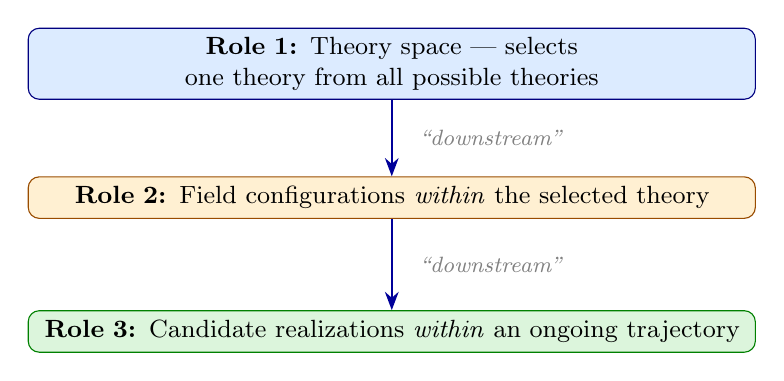
\begin{tikzpicture}[
  box/.style={draw, rounded corners=4pt, text width=9cm, align=center,
              minimum height=1.5em, font=\small},
  arrow/.style={-Stealth,thick,blue!60!black}
]
\node[box, fill=boxblue, draw=blue!50!black] (role1) at (0,0)
  {\textbf{Role 1:} Theory space — selects one theory from all possible theories};
\node[box, fill=boxorange, draw=orange!60!black] (role2) at (0,-1.7)
  {\textbf{Role 2:} Field configurations \emph{within} the selected theory};
\node[box, fill=boxgreen, draw=green!50!black] (role3) at (0,-3.4)
  {\textbf{Role 3:} Candidate realizations \emph{within} an ongoing trajectory};
\draw[arrow] (role1) -- (role2)
  node[font=\footnotesize\itshape,text=gray,right=2mm,midway] {``downstream''};
\draw[arrow] (role2) -- (role3)
  node[font=\footnotesize\itshape,text=gray,right=2mm,midway] {``downstream''};
\end{tikzpicture}
\end{center}

Role~2 cannot be applied before Role~1 (you need the selected theory before you can
vary its fields).  Role~3 cannot be applied before Role~2 (you need the dynamics
before you can specify candidate realizations).  No role refers back to any other.
There is no loop.

\begin{tcolorbox}[colback=boxblue,colframe=blue!40!black,
  title=Analogy: energy conservation]
Energy conservation governs what equilibrium configurations exist, how systems evolve
dynamically, and what energy measurements yield.  Nobody calls this circular: the same
mathematical principle manifests at multiple physical levels without any of them
referring back to the others.  MDL in GTE works the same way.
\end{tcolorbox}

The joint non-circularity is machine-certified: \lean{mdl\_tower\_three\_levels\_non\_circular}
(MDLTower.lean, ugp-lean, CatAL, zero sorry) proves that the three role certifications
hold simultaneously and that their domains are logically disjoint.

%═════════════════════════════════════════════════════════════════════════════
\section{Why This Is Remarkable}
\label{sec:remarkable}
%═════════════════════════════════════════════════════════════════════════════

\subsection{Comparison to the alternatives}

It is worth stepping back and comparing the PSC/MDL approach to the other proposed
solutions to the ``why these laws?'' problem.

\bigskip
{\setlength{\emergencystretch}{5em}\small\sloppy
\noindent\begin{tabularx}{\textwidth}{@{}p{2.6cm}p{3.2cm}p{3.2cm}X@{}}
\toprule
\textbf{Approach} & \textbf{Free parameters} & \textbf{Selection principle} & \textbf{Derives structure?} \\
\midrule
Standard Model (as usually taught)
  & 25 (measured, unexplained)
  & None
  & No — fitted to data \\[4pt]
String landscape
  & $\sim10^{500}$ vacua; ours is one
  & Anthropic (observers exist)
  & No — no mechanism \\[4pt]
Mathematical Universe (Tegmark)
  & All mathematical structures
  & Unclear; no rule
  & No — all equally real \\[4pt]
GTE/PSC/MDL
  & Zero (all derived internally)
  & PSC $\to$ PI $\equiv$ MDL
  & Yes: SM gauge structure, $N_{\rm gen}$, masses, forces \\
\bottomrule
\end{tabularx}
}

\bigskip

The crucial difference is the third column: \textbf{GTE offers a derivation, not an
assumption}.  The Standard Model says ``three generations of fermions.''
GTE says \emph{why} three, from a principle that has no adjustable parts.

\subsection{What ``derive'' means here}

To be precise: the GTE derivation is conditional.  The main named conditions are:

\begin{enumerate}[leftmargin=2em,itemsep=4pt]
\item \textbf{TSpace:} We work within four-dimensional renormalizable gauge QFT with
  compact gauge groups and chiral matter.  Gravitational extensions are handled separately.

\item \textbf{GEM (Generation-Extension Monotonicity):} Adding a generation strictly
  increases the Kolmogorov complexity of the theory.  This is well-motivated and
  accepted at CatAD but not yet Lean-certified.

\item \textbf{The PSC axiom package itself:} PSC is argued to be logically necessary
  for any fundamental theory; the argument is philosophical, not machine-certified.
\end{enumerate}

A derivation conditional on explicitly named assumptions is still a derivation — just
one with honest labeling.  The claim is not ``here is the truth''; the claim is
``here is what follows from PSC, and here is exactly what PSC assumes.''

\subsection{The number 19}

One concrete illustration of how MDL works in practice is the 19-bit count.

The GTE cellular automaton rule $p(L,C,R) = C + R - CR - LCR$ can be described in
exactly 19 bits:

\medskip
\begin{center}
\begin{tabular}{@{}lll@{}}
\toprule
\textbf{Component} & \textbf{Bits} & \textbf{What it specifies} \\
\midrule
Binary truth table (Rule 110) & 8  & The $2^3 = 8$ binary input–output pairs \\
Prime modulus $7$             & 3  & $\lceil \log_2 7 \rceil = 3$ bits \\
Monomial selector             & 5  & Which of the 8 basis monomials are nonzero \\
Chirality                     & 1  & Left–right orientation \\
Sign of nonzero coefficients  & 2  & Both nonzero non-unit coefficients are $-1$ \\
\midrule
\textbf{Total}                & \textbf{19} & \\
\bottomrule
\end{tabular}
\end{center}

\medskip

A naive lookup table specifying the same rule for all $7^3 = 343$ input combinations
requires $343 \times \lceil \log_2 7 \rceil \approx 963$ bits — about \textbf{50 times
more information}.  No other rule that reproduces the Standard Model physics can be
described in fewer than 19 bits.  This MDL uniqueness is machine-certified:
\lean{mdl\_ca\_rule\_coding\_closed} (ugp-lean, CatAL, zero sorry).

MDL is not choosing the rule because it is short.  It is recognizing that the rule's
shortness \emph{is the evidence} that it contains no redundant external choices.
A 963-bit description would contain 944 bits that came from outside the structure.
Those bits would be unexplained external inputs — free parameters by another name.
The 19-bit description has no such surplus.

\subsection{What the framework has actually derived}

To give a sense of scale: starting from the PSC axioms and MDL selection, with zero
free parameters fitted to experiment, the GTE framework derives:

\begin{itemize}[itemsep=3pt]
  \item All 9 charged-fermion masses (0.295\% RMS vs.\ PDG 2022)
  \item The electroweak mixing angle (Weinberg angle)
  \item The strong CP angle $\theta_{\rm QCD} = 0$ exactly (three independent derivations)
  \item The fine-structure constant $\alpha^{-1} = 137$ at tree level
  \item That spacetime has exactly $3{+}1$ dimensions (Lean-certified)
  \item Einstein's equations from a variational principle
  \item Newton's constant $G_N$ to 0.040\% from orbit arithmetic
  \item The Born rule for quantum probabilities (four independent derivations, two Lean-certified)
  \item The cosmological constant bracket (enclosing the Planck 2018 observed value)
\end{itemize}

None of these quantities are inputs.  They are all outputs of the PSC/MDL selection
chain.

%═════════════════════════════════════════════════════════════════════════════
\section{What PSC Leaves Open}
\label{sec:open}
%═════════════════════════════════════════════════════════════════════════════

PSC is not a theory of everything in the sense of answering every possible question.
Intellectual honesty requires stating clearly what it does and does not claim.

\begin{tcolorbox}[colback=boxgray,colframe=gray!50!black,
  title=What PSC does NOT claim to derive,breakable]
\begin{enumerate}[leftmargin=1.5em,itemsep=6pt]

\item \textbf{The strength of PSC itself.}
The claim that PSC is the correct foundation for a fundamental theory is argued
philosophically — the regress argument (\S\ref{sec:puzzle}) — not machine-certified.
Critics retain the option of accepting brute facts as legitimate components of
fundamental physics.  That is a philosophical position, not a logical error.

\item \textbf{The choice of TSpace.}
The Layer~I result holds within four-dimensional renormalizable gauge QFT.
Why should fundamental physics be described by 4D renormalizable QFT in the first
place?  The GTE framework answers this with the Dimensional Protocol Principle
(DPP) — showing that $3{+}1$ spacetime dimensions are \emph{forced} by the
dynamics — but extending this to full quantum gravity remains an open problem.

\item \textbf{The Generation-Extension Monotonicity Assumption (GEM).}
The Layer~II result (that $N_{\rm gen} = 3$ is uniquely selected) relies on GEM:
the claim that adding a generation always increases the description length of the
theory.  GEM is strongly motivated and accepted at CatAD, but a formal Lean proof
is not yet available.

\item \textbf{The absolute value of the cosmological constant.}
GTE brackets the observed value of $\Omega_\Lambda$ and provides a consistency
argument, but a full derivation of the cosmological constant from PSC alone
remains work in progress.

\item \textbf{Predictions beyond the Standard Model.}
PSC forces the SM gauge structure.  It does not, by itself, predict which specific
BSM physics (dark matter candidates, neutrino Majorana mass, proton decay rates)
is realized.  Those require further structure within the GTE dynamical framework.
\end{enumerate}
\end{tcolorbox}

The open items are genuine open problems, not rhetorical humility.  Each represents
a concrete technical task with a specific criterion for closure — Lean certification,
a specific numerical result, or a formal derivation.

\bigskip
\begin{tcolorbox}[colback=boxblue,colframe=blue!40!black,
  title=Where to go next]
\textbf{This tutorial covered:}
\begin{itemize}[itemsep=2pt]
  \item The motivation for PSC: the regress problem in physical law selection
  \item The five Layer~I axioms and what each eliminates
  \item The Two-Layer Theorem: $34{,}560 \to 12 \to 1$
  \item How PI $\equiv$ MDL terminates the regress
  \item MDL's three non-circular roles in GTE
  \item What PSC honestly leaves open
\end{itemize}

\textbf{Full treatment:} P48 monograph — all derivations, Lean certifications, and
chain diagrams — at
\href{https://doi.org/10.5281/zenodo.20560550}{doi.org/10.5281/zenodo.20560550}.

\textbf{Sister tutorial:} \emph{The GTE Polynomial: A Step-by-Step Cheat Sheet}~\cite{SpivackTutorialPolynomial} —
how the 19-bit rule produces the SM particle masses.

\textbf{Research overview:} \href{https://novaspivack.com/research}{novaspivack.com/research}
\end{tcolorbox}

%─── Acknowledgements ────────────────────────────────────────────────────────
\bigskip
\noindent\textbf{AI Disclosure.}
This tutorial was drafted with the assistance of a large-language model coding
assistant (Cursor/Claude, Anthropic), used for LaTeX composition and structural
organization.  All physics content, derivations, and claims trace to the cited papers
and machine-certified Lean proofs.  The author accepts full responsibility for
accuracy.


\section*{Further Reading}
\begin{tcolorbox}[colback=orange!8,colframe=orange!50!black,
  title=\textbf{Primary Sources}]
The results in this tutorial are derived in the following papers,
all available open-access on Zenodo and at
\href{https://novaspivack.com/research}{novaspivack.com/research}:
\begin{itemize}
  \item \textbf{P48 --- The Complete GTE Framework} (main synthesis monograph, includes
        full PSC and MDL treatment):\\
        \href{https://doi.org/10.5281/zenodo.20560550}{doi.org/10.5281/zenodo.20560550}
  \item \textbf{P01 --- Standard Model Parameters from the UGP}:\\
        \href{https://doi.org/10.5281/zenodo.20168787}{doi.org/10.5281/zenodo.20168787}
\end{itemize}
Lean~4 machine proofs: \href{https://github.com/novaspivack/ugp-lean}{github.com/novaspivack/ugp-lean}
\end{tcolorbox}

\bibliography{../../papers/bib/Spivack_Papers_Bibliography}
\end{document}
